\documentclass[12pt]{article}
\usepackage[utf8]{inputenc}
\usepackage{geometry}
\usepackage{SIunits}
\usepackage{graphicx}
\usepackage{booktabs}
\usepackage{listings}
\usepackage{color}
\usepackage{placeins}
\usepackage{rotating}
\usepackage[hidelinks]{hyperref}
\usepackage{tikz}
\usepackage{fullpage}
\usepackage{rotating}

\usetikzlibrary{shapes.geometric, arrows, positioning}
\definecolor{mygreen}{rgb}{0, 0.25, 0}
\lstset{
    tabsize = 2,
    breaklines = true,
    commentstyle = \color{mygreen} \bfseries,
    keywordstyle = \color{blue}  \bfseries,
    frame = single,
    numberstyle = \color{red}  \bfseries,
    captionpos = b,
    basicstyle = \ttfamily\footnotesize,
    language = verilog
}

\begin{document}

\begin{titlepage}
    \center
    \qquad\\[7cm]
    \textsc{\huge \bfseries Laboratory Exercise B} \\[.5cm]
    \textsc{\huge \bfseries Programmable Processor} \\[1.0cm]
    {\large TCES330 Digital Systems Design} \\[.5cm]
    {\large Spring 2014} \\[1.5cm]
    
    \begin{tabular}{ll}
        \multicolumn{2}{l}{\textbf{Authors:}}   \\
        Chad Condon:        & \underline{\hspace{5cm}} \\
        Brian Crabtree:     & \underline{\hspace{5cm}} \\
        Ben Foster:         & \underline{\hspace{5cm}} \\
        Aaron Stephens:     & \underline{\hspace{5cm}} \\
        Submission Date:    & June 6, 2014
    \end{tabular}
    
\end{titlepage}

\tableofcontents
\pagebreak

\section*{Laboratory Assignment 2} \addcontentsline{toc}{section}{Laboratory Assignment 2} \FloatBarrier

The purpose of this exercise is to build and implement a six-instruction programmable processor.
The instructions set is as shown in \hyperref[tab:instructions]{Table \ref*{tab:instructions} }.\footnote{$r$'s and $d$'s represent register file locations and data memory locations respectively.}

\begin{table}[htbp]
    \centering
    \begin{tabular}{ll}                                                                                                                 \\\toprule
        \textbf{Operation}  & \textbf{Instruction}                                                                                      \\\midrule
        NOOP                & $0000 \;\: 0000 \;\: 0000 \;\: 0000$                                                                      \\
        STORE               & $0001 \;\: r_3 r_2 r_1 r_0 \;\: d_7 d_6 d_5 d_4 d_3 d_2 d_1 d_0$                                          \\
        LOAD                & $0010 \;\: d_7 d_6 d_5 d_4 d_3 d_2 d_1 d_0 \;\: r_3 r_2 r_1 r_0$                                          \\
        ADD                 & $0011 \;\: r_{a3} r_{a2} r_{a1} r_{a0} \;\: r_{b3} r_{b2} r_{b1} r_{b0} \;\: r_{c3} r_{c2} r_{c1} r_{c0}$ \\
        SUBTRACT            & $0100 \;\: r_{a3} r_{a2} r_{a1} r_{a0} \;\: r_{b3} r_{b2} r_{b1} r_{b0} \;\: r_{c3} r_{c2} r_{c1} r_{c0}$ \\
        HALT                & $0101 \;\: 0000 \;\: 0000 \;\: 0000$                                                                      \\\bottomrule
    \end{tabular}
    \caption{Instruction Set}
    \label{tab:instructions}
\end{table}

The switches of the DE2 board are to be used as the circuit’s input, and the 7 segment displays are to be used for output.

\FloatBarrier \section{Requirements} \label{sec:requirements}

\begin{itemize}
    \item Implement the six-instruction programmable processor described in
    \href{https://moodle.insttech.washington.edu/mod/resource/view.php?id=32929}{Lecture 16b} using Verilog.
    \item Your Quartus project should be in a folder called \verb|LabB| and your top-level module should be called \verb|LabB|.
    Your top-level module will instantiate your processor module and interface to the DE2 board as follows:
    \begin{itemize}
        \item \verb|KEY[0]| acts as your system clock.
        \item \verb|KEY[1]| acts as a synchronous system reset.\footnote{%
            Note that reset will not be able reload memory contents,
            but it should reinitialize your state machine and reset (clear) \underline{all} your registers.
        }
        \item Several internal variables are brought to the top-level for debug and display purposes.
        These include the program counter, the instruction register, state machine current state,
        both inputs to the ALU, the ALU output, the contents of Register File 0, the output of the datapath multiplexer.
        \item \verb|HEX3|, \verb|2|, \verb|1|, and \verb|0| displays the current contents of the IR.
        \item \verb|SW[17:15]| determines what \verb|HEX7|, \verb|6|, \verb|5|, and \verb|4| display as follows:
        \begin{itemize}
            \item 0: \verb|HEX7| = 0; \verb|HEX6|, \verb|HEX5| = PC; \verb|HEX4| = Current State;
            \item 1: \verb|HEX7|, \verb|6|, \verb|5|, \verb|4| = ALU\_A (A-side input to ALU)
            \item 2: \verb|HEX7|, \verb|6|, \verb|5|, \verb|4| = ALU\_B (B-side input to ALU)
            \item 3: \verb|HEX7|, \verb|6|, \verb|5|, \verb|4| = ALU\_Out (ALU output)
            \item 4: Unused (use this for your own debug information)
            \item 5: \verb|HEX7|, \verb|6|, \verb|5|, \verb|4| = Register File 0 contents
            \item 6: \verb|HEX7|, \verb|6|, \verb|5|, \verb|4| = Datapath Multiplexer output
            \item 7: Unused (use this for your own debug information)
        \end{itemize}
    \end{itemize}

    \item A suggested signature for your Processor module:

    \begin{lstlisting}
module Processor( Clk, Reset, IR_Out, PC_Out, StateO, ALU_A, ALU_B, ALU_Out, RQ0, Mux_out);
    input Clk;              // system clock
    input Reset;            // system reset
    output [15:0] IR_Out;   // Instruction register
    output [4:0] PC_Out;    // Program counter
    output [3:0] StateO;    // FSM current state
    output [15:0] ALU_A;    // ALU A-Side Input
    output [15:0] ALU_B;    // ALU B-Side Input
    output [15:0] ALU_Out;  // ALU current output
    output [15:0] RQ0;      // RF[0] contents
    output [15:0] Mux_out;  // Datapath mux output
    \end{lstlisting}

    Feel free to add debug outputs to your processor module.

    \item Turn in the following sample program compiled and loaded into Instruction Memory:

    \begin{lstlisting}[numbers=none]
RF[0] = D[A] - D[1A] + D[3] - D[8A];
D[BB] = RF[0];
HALT
    \end{lstlisting}

    Data memory should contain:

    \begin{lstlisting}[numbers=none]
D[3] = 0x10AA
D[A] = 0xB0C5
D[1A] = 0x00DC
D[8A] = 0x00E9
    \end{lstlisting}
    \item Make sure that the In System Memory Content Editor can display the contents of both of your memories.
    \item Make sure Quartus recognizes your state machine (as a state machine).
    \item Data memory should be a $256 \times 16$ Quartus RAM LPM with Memory Content Editor enabled.
    \item The Register File should be from Homework 6.
    \item The ALU should be from Homework 6.
    \item The Instruction memory should be a $32 \times  16$ Quartus ROM LPM with Memory Content Editor enabled.
    \item The controller state machine should be similar to the one shown in Lecture 16b.
    \item Implement a ModelSim testbench project that exercises your processor with the required program.
    You may wish to test with additional programs,
    but the \verb|*.mif| files you turn in should contain the instructions
    and data necessary to implement the program shown above.
    \item Write your report using the same outline as before.
    You know by now to be very explicit and detailed about your test procedure and test results.
    Photographs are allowed.
\end{itemize} \FloatBarrier \clearpage
\FloatBarrier \section{Design} \label{sec:design}

Analysis of the requirements described in \hyperref[sec:requirements]{Section \ref*{sec:requirements}} as well as those in \href{https://moodle.insttech.washington.edu/mod/resource/view.php?id=32929}{Lecture 16b} yielded the hierarchy shown in \hyperref[fig:hierarchy]{Figure \ref*{fig:hierarchy}}.
The design of each module will be discussed below.

\begin{figure}[htbp]
    \center
    \begin{center}
    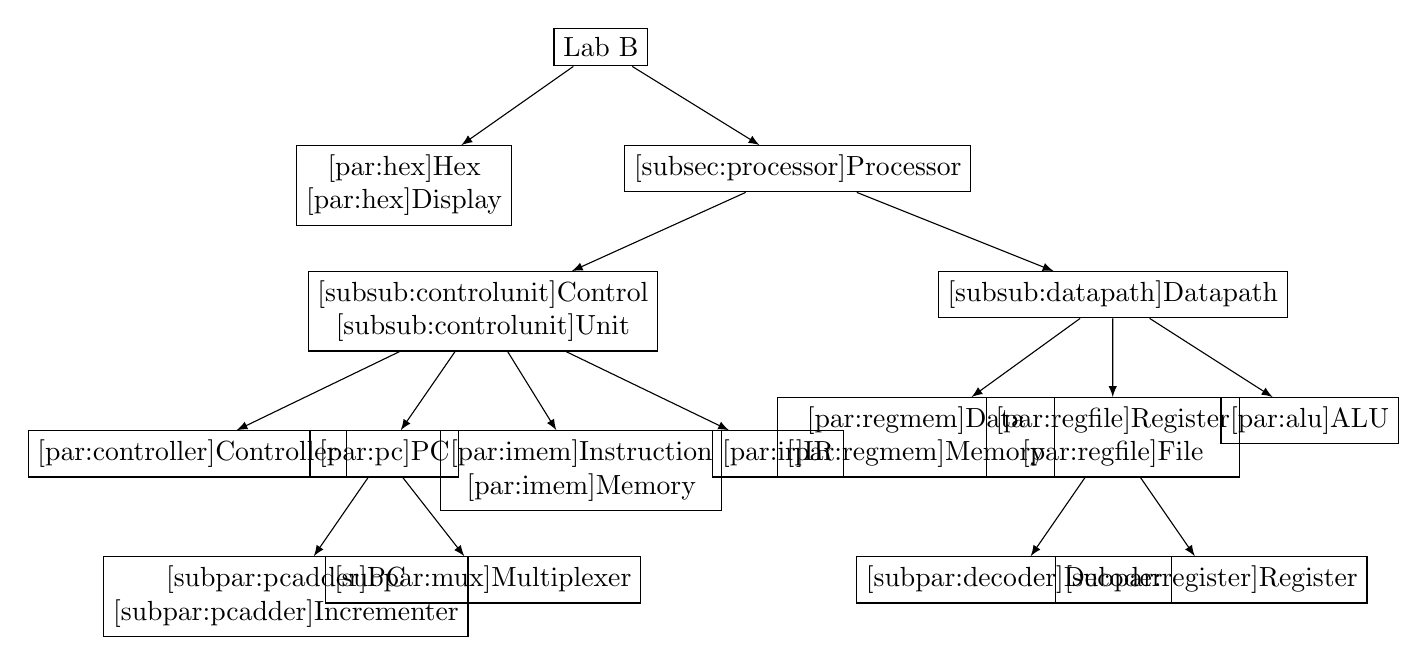
\begin{tikzpicture}[
            every node/.style = {rectangle, align = center},
            level/.style = {growth parent anchor = south, level distance = 1cm},
            level 1/.style = {sibling distance = 5cm},
            level 2/.style = {sibling distance = 8cm},
            level 3/.style = {sibling distance = 2.5cm},
            level 4/.style = {sibling distance = 2.5cm},
            edge from parent/.style = {draw,-latex},
            every child node/.style = {anchor = north}]
        \node [draw] (top) {Lab B}
            child {node [draw] (Hex7Seg) {
                \hyperref[par:hex]{Hex} \\
                \hyperref[par:hex]{Display}}
            }
            child {node [draw] (Processor) {\hyperref[subsec:processor]{Processor}}
                child {node [draw] (cunit) {
                    \hyperref[subsub:controlunit]{Control} \\
                    \hyperref[subsub:controlunit]{Unit}
                }
                    child {node [draw] (controller) {\hyperref[par:controller]{Controller}}}
                    child {node [draw] (PC) {\hyperref[par:pc]{PC}}
                        child {node [draw] (PCAdderer) {
                            \hyperref[subpar:pcadder]{PC} \\
                            \hyperref[subpar:pcadder]{Incrementer}}
                        }
                        child {node [draw] (PCUp) {\hyperref[subpar:mux]{Multiplexer}}}
                    }
                    child {node [draw] (imemlpm) {
                        \hyperref[par:imem]{Instruction} \\
                        \hyperref[par:imem]{Memory}}
                    }
                    child {node [draw] (IR) {\hyperref[par:ir]{IR}}}
                }
                child {node [draw] (Datapath) {\hyperref[subsub:datapath]{Datapath}}
                    child {node [draw] (RAM) {
                        \hyperref[par:regmem]{Data} \\
                        \hyperref[par:regmem]{Memory}}
                    }
                    child {node [draw] (RegisterFile) {
                        \hyperref[par:regfile]{Register} \\
                        \hyperref[par:regfile]{File}
                    }
                    child {node [draw] (PCClear) {\hyperref[subpar:decoder]{Decoder}}}
                        child {node [draw] (Register) {\hyperref[subpar:register]{Register}}}
                    }
                    child {node [draw] (ALU) {\hyperref[par:alu]{ALU}}}
                }
            };
    \end{tikzpicture}
    \end{center}
    \caption{Design Hierachy \label{fig:hierarchy}}
\end{figure}

The top-level module must have the properties listed below.

\begin{itemize}
    \item One one-bit input $KEY_0$ as the clock signal.
    \item One one-bit input $KEY_1$ as the active low reset signal.
    \item One two-bit input $SW_{17:15}$ as the display select signal.
    \item Four seven-bit outputs $HEX0$, $HEX1$, $HEX2$, and $HEX3$ as the instruction display.
    \item Four seven-bit outputs $HEX4$, $HEX5$, $HEX6$, and $HEX7$ as selectable display.
    \item The value of $SW_{17:15}$ selects the value to be displayed on $HEX4$, $HEX5$, $HEX6$, and $HEX7$ as shown in
    \hyperref[tab:display]{Table \ref*{tab:display}}.
\end{itemize}

\begin{table}[htbp]
    \center
    \begin{tabular}{ll}                             \toprule
        $SW_{17:15}$    & Displayed Values              \\\midrule
        0               & Current State                 \\
        1               & A side input to ALU           \\
        2               & B side input to ALU           \\
        3               & ALU output                    \\
        4               & \emph{Unused}                 \\
        5               & Register File 0 contents      \\
        6               & Datapath multiplexer output   \\
        7               & \emph{Unused}                 \\\bottomrule
    \end{tabular}
\caption{Selectable Display Values\label{tab:display}}
\end{table}

The file \verb|LabB.v| contains the module \verb|LabB| which satisfies these properties.
A listing can be found in \hyperref[lst:LabB]{Listing \ref*{lst:LabB}} in the \hyperref[sec:appendix]{Appendix}.Also note that the necessary pin assignments can be found in\hyperref[lst:pins]{Listing \ref*{lst:pins}} in the \hyperref[sec:appendix]{Appendix}.

\paragraph{Hex Display} \label{par:hex}

The top-level module required a hex display Verilog module with the properties listed below.
This module was reused from Homework 2.

\begin{itemize}
    \item One four-bit input $C$ as the displayed value.
    \item One seven-bit output $Display$ as the seven segment display.
    \item Assigns $Display$ to the value that displays the hexadecimal character representing $C$'s value on a seven segment display.
\end{itemize}

The file \verb|Hex7seg.v| contains the module \verb|Hex7seg| which satisfies these properties.
A listing can be found in \hyperref[lst:hex]{Listing \ref*{lst:hex}} in the \hyperref[sec:appendix]{Appendix}.

\subsection{Processor}  \label{subsec:processor}

The top-level module required a processesor Verilog modules with the properties listed below.

\begin{itemize}
    \item One one-bit input $Clk$ as the clock signal.
    \item One one-bit input $Reset$ as the active high reset signal.
    \item One sixteen-bit output $IR_\text{Out}$ as the instruction register value.
    \item One five-bit output $PC_\text{Out}$ as the program counter value.
    \item One four-bit output $State0$ as the current state.
    \item Two sixteen-bit outputs $ALU_A$ and $ALU_B$ as the A- and B-side ALU inputs respectively.
    \item One sixteen-bit output $ALU_\text{Out}$ as the ALU output.
    \item One sixteen-bit output $RQ0$ as the register file 0 entry.
    \item One sixteen-bit output $Mux_\text{out}$ as the datapath multiplexer output.
\end{itemize}

The file \verb|Processor.v| contains the module \verb|Processor| which satisfies these properties.
A listing can be found in \hyperref[lst:processor]{Listing \ref*{lst:processor}} in the \hyperref[sec:appendix]{Appendix}.

\subsubsection{Control Unit} \label{subsub:controlunit}

The processor module required a control unit Verilog module with the properties listed below.

\begin{itemize}
    \item One one-bit input $Clock$ as the clock signal.
    \item One eight-bit output $D_text{addr}$ as the data memory address.
    \item One four-bit output $RF_{W_\text{addr}}$ as the register file write address.
    \item Two four-bit outputs $RF_{Ra_\text{addr}}$ and $RF_{Rab_\text{addr}}$ as the register file A
    and B stream read addresses respectively.
    \item One one-bit output $D_\text{wr}$ as the data memory write enable signal.
    \item One one-bit output $RF_s$ as the data multiplexer select signal.
    \item One three-bit output $Alu_{s0}$ as the ALU function select signal.
    \item One one-bit output $RF_{W_\text{wr}}$ as the register file write enable signal.
    \item Two one-bit inputs $RF_{Ra_\text{rd}}$ and $RF_{Rab_\text{rd}}$ as the register file A and B
    stream read enable signals respectively.
    \item One One five-bit output $RC_\text{Out}$ as the program counter address.
    \item One sixteen-bit output $IR_\text{Out}$ as the current instruction.
    \item One four-bit output $State0$ as the controller state.
\end{itemize}

The file \verb|cunit.v| contains the module \verb|cunit| which satisfies these properties.
A listing can be found in \hyperref[lst:cunit]{Listing \ref*{lst:cunit}} in the \hyperref[sec:appendix]{Appendix}.

\paragraph{Program Counter} \label{par:pc}

The control unit module required a program counter Verilog module with the properties listed below.

\begin{itemize}
    \item One one-bit input $Clear$ as the active high, synchronous clear signal.
    \item One one-bit input $Up$ as the load enable signal.
    \item One one-bit input $Clock$ as the clock signal.
    \item One five-bit output $O$ as the program counter value.
\end{itemize}

The file \verb|PC.v| contains the module \verb|PC| which satisfies these properties.
A listing can be found in \hyperref[lst:pc]{Listing \ref*{lst:pc}} in the \hyperref[sec:appendix]{Appendix}.

\subparagraph{PC Incrementer} \label{subpar:pcadder}

The program counter module required a PC incrementer Verilog module with the properties listed below.

\begin{itemize}
    \item One five-bit input $I$.
    \item One five-bit output $O$ which passes the sum $I + 1$.
\end{itemize}

The file \verb|PCAdder.v| contains the module \verb|PCAdder| which satisfies these properties.
A listing can be found in \hyperref[lst:PCAdder]{Listing \ref*{lst:PCAdder}} in the \hyperref[sec:appendix]{Appendix}.

\subparagraph{Multiplexer} \label{subpar:mux}

The program counter module required an multiplexer Verilog module with the properties listed below.

\begin{itemize}
    \item Two five-bit inputs $data0x$ and $data1x$ as the selectable inputs.
    \item One one-bit input $sel$ as the select signal.
    \item One one-bit output $result$ which passes $data0x$ or $data1x$ if $sel$ is 0 or 1 respectively.
\end{itemize}


The file \verb|muxlpm.v| contains the module \verb|muxlpm| which satisfies these properties from the \emph{Altera} library of parameterized modules.
A listing can be found in \hyperref[lst:muxlpm]{Listing \ref*{lst:muxlpm}} in the \hyperref[sec:appendix]{Appendix}.

\paragraph{Instruction Register} \label{par:ir}

The control unit module required an instruction register Verilog module with the properties listed below.

\begin{itemize}
    \item Parameterized data bit width $N$.
    \item One one-bit input $clk$ as the clock signal.
    \item One $N$-bit input $d$ as the input value.
    \item One one-bit input $ir_\text{ld}$ as the load enable signal.
    \item One $N$-bit output $q$ as the register's value.
\end{itemize}

The file \verb|instruction_register.v| contains the module \verb|instruction_register| which satisfies these properties.
A listing can be found in \hyperref[lst:ir]{Listing \ref*{lst:ir}} in the \hyperref[sec:appendix]{Appendix}.

\paragraph{Controller} \label{par:controller}

The control unit module required controller Verilog module with the properties listed below.

\begin{itemize}
    \item One sixteen-bit input $instruction$ which accepts an intruction.
    \item One one-bit input $clk$ which acts as the clock.
    \item One one-bit output $PC_\text{clr}$ which signals to clear the program counter.
    \item One one-bit output $PC_\text{up}$ which signals to increment to program counter.
    \item One one-bit output $IR_\text{ld}$ which signals to load the instruction register.
    \item One one-bit output $RF_\text{s}$ which selects the register file.
    \item One one-bit output $RF_{W_\text{wr}}$ which signals to write enable the register file.
    \item One one-bit output $RF_{Ra_\text{rd}}$ which signals to read enable the A stream of the register file.
    \item One one-bit output $RF_{Rb_\text{rd}}$ which signals to read enable the B stream of the regoster file.
    \item One eight-bit output $D_\text{addr}$ which signals the data memory address.
    \item One one-bit output $D_{wr}$ which signals to write enable the data memory.
    \item One four-bit output $RF_{W_\text{addr}}$ which signals the register file's write address.
    \item One four-bit output $RF_{Ra_\text{addr}}$ which signals the register file's A stream read address.
    \item One four-bit output $RF_{Rb_\text{addr}}$ which signals the register files' B stream read address.
    \item One four-bit output $Alu_\text{s0}$ which selects the arithmetic logic unit's function.
    \item One four-bit output $State$ which signals the current state,
    \item Positive edge triggered.
    \item Quartus recognized state machine.
    \item Ten states representing each phase of each instruction.\footnote{%
        See \hyperref[tab:instructions]{Table \ref*{tab:instructions}} for a list of instructions.
    }
    \begin{itemize}
        \item \textbf{INIT}: Wait
        \item \textbf{FETCH}: Retrieve new instruction
        \item \textbf{DECODE}: Interpret instruction
        \item \textbf{NOOP}: Do nothing
        \item \textbf{LOAD\_A}: Begin load operation
        \item \textbf{LOAD\_B}: Complete load operation
        \item \textbf{STORE}: Store operation
        \item \textbf{ADD}: Addition operation
        \item \textbf{SUB}: Substraction operation
        \item \textbf{HALT}: Stop all operations
    \end{itemize}
\end{itemize}

The file \verb|controller.v| contains the module \verb|controller| which satisfies these properties.
A listing can be found in \hyperref[lst:controller]{Listing \ref*{lst:controller}} in the \hyperref[sec:appendix]{Appendix}.

\paragraph{Instruction Memory} \label{par:imem}

The control unit module required an instruction memory Verilog module with the properties listed below.

\begin{itemize}
    \item One five-bit input $address$ as the data address.
    \item One one-bit input $clock$ as the clock signal.
    \item One sixteen-bit output $q$ as the data read signal.
    \item Loaded with the instructions described in \hyperref[sec:requirements]{Section \ref*{sec:requirements}}
\end{itemize}

The file \verb|imemlpm.v| contains the module \verb|imemlpm| which satisfies these properties from the \emph{Altera} library of parameterized modules.
A listing can be found in \hyperref[lst:imemlpm]{Listing \ref*{lst:imemlpm}} in the \hyperref[sec:appendix]{Appendix}.
A listing of the Memory Instantiation File can be found in \hyperref[lst:imemmif]{Listing \ref*{lst:imemmif}} in the \hyperref[sec:appendix]{Appendix}.

\subsubsection{Datapath} \label{subsub:datapath}

The processor module required datapath Verilog module with the properties listed below.

\begin{itemize}
    \item One one-bit input $Clock$ as the clock signal.
    \item One one-bit input $Reset$ as an active high, synchronous reset signal.
    \item One eight-bit input $D_\text{addr}$ as the data memory address.
    \item One one-bit input $D_\text{wr}$ as the data memory write enable signal.
    \item One four-bit input $RF_{W_\text{addr}}$ as the register file write address.
    \item One one-bit input $RF_{W_\text{wr}}$ as the register file write enable signal.
    \item One four-bit input $RF_{Ra_\text{addr}}$ as the register file stream A read address.
    \item One one-bit input $RF_{Ra_\text{rd}}$ as the register file stream A read enable signal.
    \item One four-bit input $RF_{Rb_\text{addr}}$ as the register file stream B read address.
    \item One one-bit input $RF_{Rb_\text{rd}}$ as the register file stream B read enable signal.
    \item One three-bit input $Alu_{s0}$ as the ALU function select signal.
    \item Two sixteen-bit outputs $ALU_A$ and $ALU_B$ as the ALU A- and B-side inputs respectively.
    \item One sixteen-bit output $RQ0$ as the first register file entry.
    \item One sixteen-bit output $Mux_\text{out}$ as register file write data input.
    \item Positive edge triggered.
\end{itemize}

The file \verb|Datapath.v| contains the module \verb|Datapath| which satisfies these properties.
A listing can be found in \hyperref[lst:datapath]{Listing \ref*{lst:datapath}} in the \hyperref[sec:appendix]{Appendix}.

\paragraph{Data Memory} \label{par:regmem}

The datapath module required register memory Verilog module with the properties listed below.
This module was reused frome Homework 6.

\begin{itemize}
    \item One eight-bit input $address$ as the read/write address.
    \item One one-bit input $clock$ as the clock signal.
    \item One sixteen-bit input $data$ as the data to write.
    \item One one-bit input $wren$ as the write-enable signal.
    \item One sixteen-bit output $q$ as the read data stream.
    \item Positive edge-triggered.
    \item $256 \times 16$ Quartus RAM LPM with Memory Content Editor enabled.
    \item Loaded with the data described in \hyperref[sec:requirements]{Section \ref*{sec:requirements}}
\end{itemize}

The file \verb|ramlpm.v| contains the module \verb|ramlpm| which satisfies these properties from the \emph{Altera} library of parameterized modules.
A listing can be found in \hyperref[lst:ramlpm]{Listing \ref*{lst:ramlpm}} in the \hyperref[sec:appendix]{Appendix}.
A listing of the Memory Instantiation File can be found in \hyperref[lst:rammif]{Listing \ref*{lst:rammif}} in the \hyperref[sec:appendix]{Appendix}.

\paragraph{Register File} \label{par:regfile}

The datapath module required a register file Verilog module with the properties listed below.
This module was reused from Homework 6.

\begin{itemize}
    \item One one-bit input $Clk$ as the clock signal.
    \item One one-bit input $Reset$ as an active high reset signal.
    \item One sixteen-bit input $W_\text{data}$ as the data to write.
    \item One four-bit input $W_\text{addr}$ as the write address.
    \item One one-bit input $W_\text{en}$ as the write enable signal.
    \item Two four-bit inputs $R_\text{addr0}$ and $R_\text{addr1}$ as the A and B stream read addresses respectively.
    \item Two one-bit inputs $R_\text{en0}$ and $R_\text{en1}$ as the A and B stream read enable signals respectively.
    \item Two sixteen-bit outputs $R_\text{data0}$ and $R_\text{data1}$ as the A and B data streams respectively.
    \item One sixteen-bit output $RQ0$ which signals the contents of register 0.
    \item Positive edge triggered.
\end{itemize}

The file \verb|RegisterFile.v| contains the module \verb|RegisterFile| which satisfies these properties.
A listing can be found in \hyperref[lst:registerfile]{Listing \ref*{lst:registerfile}} in the \hyperref[sec:appendix]{Appendix}.

\subparagraph{Decoder} \label{subpar:decoder}

The register file module required a decoder Verilog module with the properties listed below.
This module was reused from Homework 6.

\begin{itemize}
    \item Parameterized input size $N$.
    \item One $N$-bit select input $W$.
    \item One one-bit enable input $E$.
    \item One $2^N$-bit output $Y$.
    \item ``One hot'' decoder with enable.
\end{itemize}

The file \verb|DecoderN.v| contains the module \verb|DecoderN| which satisfies these properties.
A listing can be found in \hyperref[lst:DecoderN]{Listing \ref*{lst:DecoderN}} in the \hyperref[sec:appendix]{Appendix}.

\subparagraph{Register} \label{subpar:register}

The register file module required a register Verilog module with the properties listed below.
This module was reused from Homework 6.

\begin{itemize}
    \item Parameterized data size $N$
    \item One one-bit input $Clk$ as the clock signal.
    \item One one-bit input $Rst$ as an active high reset.
    \item One one-bit input $Ld$ as a load enable signal.
    \item One one-bit input $Oe0$ as the A stream output enable signal.
    \item One one-bit input $Oe1$ the B stream output enable signal.
    \item One $N$-bit input $I$ as the data to load.
    \item One $N$-bit output $Qz0$ as the switched A stream switched output.
    \item One $N$-bit output $Qz1$ as the switched B stream switched output.
    \item One $N$-bit output $QR$ as the the unswitched output.
    \item Positive edge triggered.
    \item Holds the value of $I$ when $Ld = 1$.
    \item Outputs the data to $Qz0$ and $Qz1$ when $Oe0$ and $Oe1$ are high respectively.
    \item Outputs high impedence otherwise.
\end{itemize}

The file \verb|RegisterOEN.v| contains the module \verb|RegisterOEN| which satisfies these properties.
A listing can be found in \hyperref[lst:RegisterOEN]{Listing \ref*{lst:RegisterOEN}} in the \hyperref[sec:appendix]{Appendix}.

\paragraph{Arithmetic Logic Unit} \label{par:alu}

The datapath module required an arithmetic logic unit Verilog module with the properties listed below.
This module was reused from Homework 6.

\begin{itemize}
    \item Two sixteen-bit inputs: $A$ and $B$.
    \item One three-bit input: $Sel$.
    \item One sixteen-bit output: $Q$.
    \item $Q$ is a function of $A$ and $B$ as selected by $Sel$ as shown in \hyperref[tab:alu]{Table \ref*{tab:alu}}..
        \begin{table}[htbp]
            \center
            \begin{tabular}{ll}             \toprule
                $Sel$       & $Q$           \\\midrule
                0           & $0$           \\
                1           & $A + B$       \\
                2           & $A - B$       \\
                3           & $A$           \\
                4           & $A \oplus B$  \\
                5           & $A \lor B$    \\
                6           & $A \land B$   \\
                7           & $A + 1$       \\\bottomrule
            \end{tabular}
            \caption{ALU output}
            \label{tab:alu}
        \end{table}
\end{itemize}

The file \verb|ALU.v| contains the module \verb|ALU| which satisfies these properties.
A listing can be found in \hyperref[lst:alu]{Listing \ref*{lst:alu}} in the \hyperref[sec:appendix]{Appendix}.
 \FloatBarrier \clearpage
\FloatBarrier \section{Test Procedures} % (fold)
\label{sec:test_procedures}

The following test procedures will be used to verify that each part of this laboratory exercise satisfies the requirements given in \hyperref[sec:requirements]{Section \ref*{sec:requirements}}.
Modules are to be tested beginning with lower-level modules and moving up so as to isolate issues in a module dependencies.

\subsection{PC Incrementer} % (fold)
\label{sub:pc_incrementer_procedure}

The following test procedure will be used to verify that the Verilog module, \verb|PCAdder|, satisfies the requirements for this part.

%TODO test PCAdder
\begin{enumerate}
    \item The PC incrementer circuit will be tested using \emph{ModelSim} and the testbench shown in \hyperref[lst:testPCAdder]{Listing \ref*{lst:testPCAdder}}.
    This testbench generates the test vectors shown in \hyperref[tab:pcadder_vectors]{Table \ref*{tab:pcadder_vectors}} and outputs the output $O$.
    Simulations will be run in order to verify the behavior shown in \hyperref[tab:pcadder_vectors]{Table \ref*{tab:pcadder_vectors}}.
    \item Generate the test vectors shown in \hyperref[tab:pcadder_vectors]{Table \ref*{tab:pcadder_vectors}} and verify the corresponding outputs, $O$.
\end{enumerate}

\begin{table}[htbp]
    \centering
        \begin{tabular}{ll} \toprule
            $I$     & $O$   \\\midrule
            00000   & 00001 \\
            00001   & 00010 \\
            00010   & 00011 \\
            00011   & 00100 \\
            00100   & 00101 \\
            00101   & 00110 \\
            00110   & 00111 \\
            00111   & 01000 \\
            01000   & 01001 \\
            01001   & 01010 \\
            01010   & 01011 \\
            01011   & 01100 \\
            01100   & 01101 \\
            01101   & 01110 \\
            01110   & 01111 \\
            01111   & 10000 \\
            10000   & 10001 \\
            10001   & 10010 \\
            10010   & 10011 \\
            10011   & 10100 \\
            10100   & 10101 \\
            10101   & 10110 \\
            10110   & 10111 \\
            10111   & 11000 \\
            11000   & 11001 \\
            11001   & 11010 \\
            11010   & 11011 \\
            11011   & 11100 \\
            11100   & 11101 \\
            11101   & 11110 \\
            11110   & 11111 \\
            11111   & 00000 \\\bottomrule
        \end{tabular}
    \caption{PC Incrementer Test Vectors\label{tab:pcadder_vectors}}
\end{table}
% subsection pc_incrementer (end)

\subsection{Multiplexer} % (fold)
\label{sub:multiplexer}

The multiplexer module, \verb|PCUp|, was implemented from the \emph{Altera} library of parameterized modules (LPM).
It will therefore not be specifically tested.

% subsection multimplexer (end)

\subsection{Decoder} % (fold)
\label{sub:decoder}

The decoder module, \verb|DecoderN|, has been previously used and tested for Homework 6.
It will therefore not be specifically tested.
% subsection decoder (end)

\subsection{Register} % (fold)
\label{sub:register}

The register module, \verb|RegisterOEN|, has been previously used and tested for Homework 6 and only minimally modified.
It will therefore not be specifically tested.
% subsection register (end)

\FloatBarrier \subsection{Controller} % (fold)
\label{sub:controller_pro}

The following test procedure will be used to verify that the Verilog module, \verb|controller|, satisfies the requirements for this part.

%TODO test controller
\begin{enumerate}
    \item The PC incrementer circuit will be tested by intputting the instrunctions shown in \hyperref[tab:controller_test_instructions]{Table \ref*{tab:controller_test_instructions}}
    each followed by a reset signal.
    Simulations will be run in order to verify the behavior shown in
    \hyperref[fig:state_diagram]{Figure \ref*{fig:state_diagram}}.
    \item Verify that the \emph{RTL Viewer} shows a state machine.
    \item Generate the behavior shown in \hyperref[fig:state_diagram]{Figure \ref*{fig:state_diagram}} and verify the corresponding outputs.
\end{enumerate}

\begin{table}
    \centering
    \begin{tabular}{ll}                                                 \toprule
        \textbf{Instruction Type}   & \textbf{Instruction}              \\\midrule
        NOOP                        & $0000 \; 0000 \; 0000 \; 0000$    \\
        STORE                       & $0001 \; 0100 \; 0000 \; 0101$    \\
        LOAD                        & $0010 \; 0000 \; 0011 \; 0100$    \\
        ADD                         & $0011 \; 0001 \; 0010 \; 0011$    \\
        SUBTRACT                    & $0100 \; 0110 \; 0101 \; 0100$    \\
        HALT                        & $0101 \; 0000 \; 0000 \; 0000$    \\\bottomrule
    \end{tabular}
    \caption{Controller Test Instructions\label{tab:controller_test_instructions}}
\end{table}

\begin{figure}
    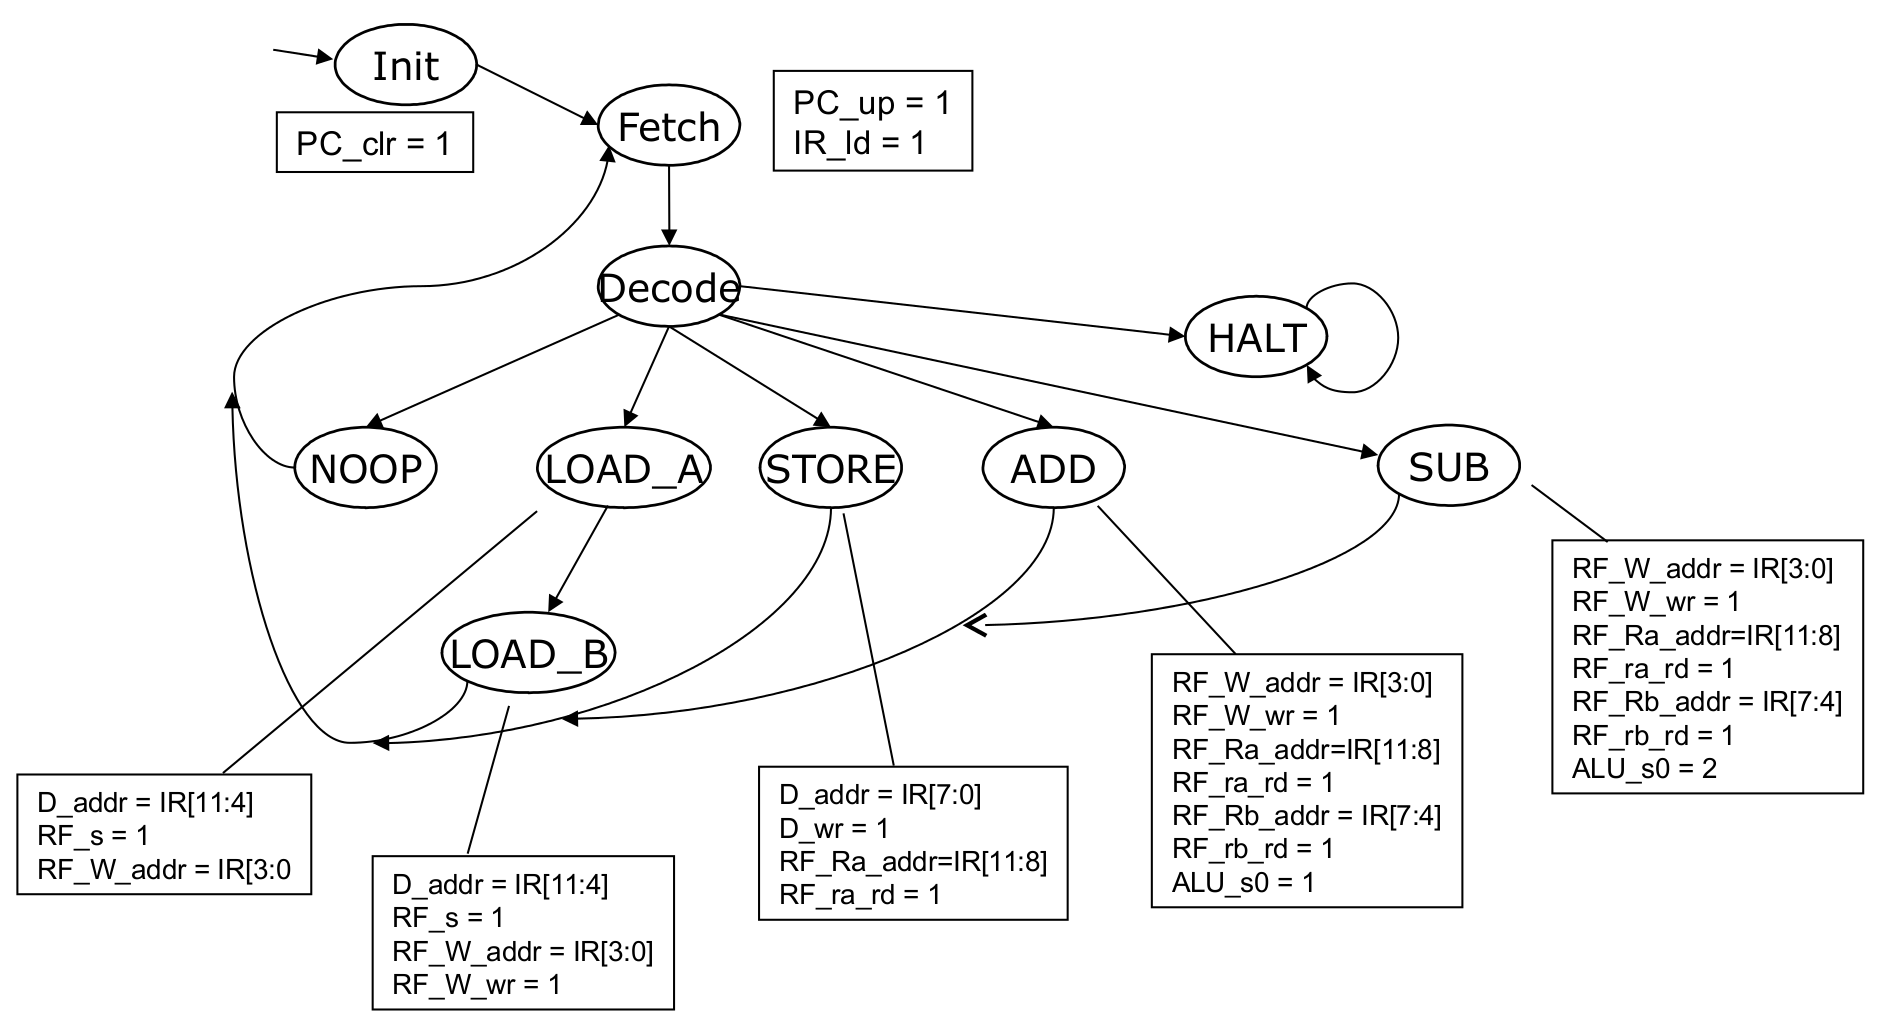
\includegraphics[width=\textwidth]{images/state_diagram.png}
    \caption{Controller State Diagram \label{fig:state_diagram}}
\end{figure}

% subsection controller (end)

\subsection{Program Counter} % (fold)
\label{sub:program_counter_pro}

The following test procedure will be used to verify that the Verilog module, \verb|PC|, satisfies the requirements for this part.

%TODO Test PC
\begin{enumerate}
    \item The program counter circuit will be tested using \emph{ModelSim} and the testbench shown in \hyperref[lst:testPC]{Listing \ref*{lst:testPC}}.
    This testbench generates the test vectors shown in \hyperref[tab:pc_vectors]{Table \ref*{tab:pc_vectors}} and output $O$.
    Simulations will be run in order to verify the behavior shown in \hyperref[tab:pc_vectors]{Table \ref*{tab:pc_vectors}}.
    \item Generate the test vectors shown in \hyperref[tab:pc_vectors]{Table \ref*{tab:pc_vectors}}
    and verify the corresponding outputs.
\end{enumerate}

\begin{table}[htbp]
    \centering
        %TODO tabular
    \caption{Program Counter Test Vectors\label{tab:pc_vectors}}
\end{table}

% subsection program_counter (end)

\subsection{Instruction Memory} % (fold)
\label{sub:instruction_memory}

The instruction memory module, \verb|imemlpm| is implemented from the LPM.
It will therefore not be specifically tested.
% subsection instruction_memory (end)


\subsection{Instruction Register} % (fold)
\label{sub:instruction_register_pro}

The following test procedure will be used to verify that the Verilog module, \verb|instruction_register|, satisfies the requirements for this part.

%TODO test control unit
\begin{enumerate}
    \item The instruction register circuit will be tested using \emph{ModelSim} and the testbench shown in %TODO Figure 9, Appendix A.
    This testbench generates the test vectors shown in \hyperref[tab:ir_vectors]{Table \ref*{tab:ir_vectors}} and output %TODO $O$.
    Simulations will be run in order to verify the behavior shown in \hyperref[tab:ir_vectors]{Table \ref*{tab:ir_vectors}}.
    \item Generate the test vectors shown in \hyperref[tab:ir_vectors]{Table \ref*{tab:ir_vectors}}
    and verify the corresponding outputs.
\end{enumerate}

\begin{table}[htbp]
    \centering
        %TODO tabular
    \caption{Control Unit Test Vectors\label{tab:ir_vectors}}
\end{table}

% subsection instruction_register (end)

\subsection{Data Memory} % (fold)
\label{sub:data_memory}

The instruction memory module, \verb|ramlpm| is implemented from the LPM.
It will therefore not be specifically tested.
% subsection data_memory (end)

\subsection{Register File} % (fold)
\label{sub:register_file}

The register file module, \verb|RegisterFile|, has been previously used and tested for Homework 6 and only minimally modified.
It will therefore not be specifically tested.
% subsection register_file (end)

\subsection{Arithmetic Logic Unit} % (fold)
\label{sub:arithmetic_logic_unit}

The arithmetic logic unit module, \verb|ALU|, has been previously used and tested for Homework 6.
It will therefore not be specifically tested.
% subsection arithmetic_logic_unit (end)

\subsection{Control Unit} % (fold)
\label{sub:control_unit_pro}

The control unit module, \verb|cunit| serves only to instantiate the controller, the program counter, the intruction memory, and the instruction register.
There is no logic contained in the module.
It will therefore not be specifically tested.

% subsection control_unit (end)

\subsection{Datapath} % (fold)
\label{sub:datapath_pro}

The datapath module, \verb|datapath| serves only to instantiate the data memory, the register file, and the arithmetic logic unit.
The only logic contained within the module is a simple two-to-one multiplexer.
It will therefore not be specifically tested.

% subsection datapath (end)

\subsection{Processor} % (fold)
\label{sub:processor_pro}

The following test procedure will be used to verify that the Verilog module, \verb|Processor|, satisfies the requirements for this part.

%TODO test processor
\begin{enumerate}
    \item The processor circuit will be tested using \emph{ModelSim} and the testbench shown in \hyperref[lst:testProcessor]{Listing \ref*{lst:testProcessor}}.
    This testbench generates the test vectors shown in \hyperref[tab:processor_vectors]{Table \ref*{tab:processor_vectors}} and output %TODO $O$.
    Simulations will be run in order to verify the behavior shown in \hyperref[tab:processor_vectors]{Table \ref*{tab:processor_vectors}}.
    \item Generate the test vectors shown in \hyperref[tab:processor_vectors]{Table \ref*{tab:processor_vectors}} and verify the corresponding outputs.
\end{enumerate}

\begin{table}[htbp]
    \centering
        %TODO tabular
    \caption{Processor Test Vectors\label{tab:processor_vectors}}
\end{table}

% subsection processor (end)

\subsection{Hex Display} % (fold)
\label{sub:hex_display}

The hex display module, \verb|Hex7seg|, has been previously used and tested for several assignments.
It will therefore not be specifically tested.
% subsection hex_display (end)

\subsection{Project} % (fold)
\label{sub:project_pro}

The following test procedure will be used to verify that the \emph{Quartus II} project \verb|Lab6| satisfies the requirements for this lab.

\begin{enumerate}
    \item Open the project and verify that compilation produces no errors or unallowed warnings.
    \item Load the project onto the DE2 board without errors.
    \item Verify that the displayed output is selected as described in \hyperref[tab:display]{Table \ref*{tab:display}}.
\end{enumerate}

% subsection project (end)

% section test_procedures (end)
 \FloatBarrier \clearpage
\FloatBarrier \section{Test Results} % (fold)
\label{sec:test_results}

\subsection{PC Incrementer} % (fold)
\label{sub:pc_incrementer}

The following observations correspond to the numbers in the \hyperref[sec:test_procedures]{Section \ref*{sec:test_procedures}} procedures for this part:

\begin{enumerate}
    \item The simulation using \emph{ModelSim} produced the output shown in \hyperref[fig:pcadder_output]{Figure \ref*{fig:pcadder_output}}.
    This output corresponds to \hyperref[tab:pcadder_vectors]{Table \ref*{tab:pcadder_vectors}} for each row, indicating the simulation passes.
    \item All test vectors as specified in \hyperref[tab:pcadder_vectors]{Table \ref*{tab:pcadder_vectors}} produced the corresponding outputs
\end{enumerate}

\begin{figure}[htbp]
    \begin{lstlisting}[numbers=none, basicstyle = \ttfamily\scriptsize]
# Time is          0 | I = 00 | O = 01
# Time is         10 | I = 01 | O = 02
# Time is         20 | I = 02 | O = 03
# Time is         30 | I = 03 | O = 04
# Time is         40 | I = 04 | O = 05
# Time is         50 | I = 05 | O = 06
# Time is         60 | I = 06 | O = 07
# Time is         70 | I = 07 | O = 08
# Time is         80 | I = 08 | O = 09
# Time is         90 | I = 09 | O = 0a
# Time is        100 | I = 0a | O = 0b
# Time is        110 | I = 0b | O = 0c
# Time is        120 | I = 0c | O = 0d
# Time is        130 | I = 0d | O = 0e
# Time is        140 | I = 0e | O = 0f
# Time is        150 | I = 0f | O = 10
# Time is        160 | I = 10 | O = 11
# Time is        170 | I = 11 | O = 12
# Time is        180 | I = 12 | O = 13
# Time is        190 | I = 13 | O = 14
# Time is        200 | I = 14 | O = 15
# Time is        210 | I = 15 | O = 16
# Time is        220 | I = 16 | O = 17
# Time is        230 | I = 17 | O = 18
# Time is        240 | I = 18 | O = 19
# Time is        250 | I = 19 | O = 1a
# Time is        260 | I = 1a | O = 1b
# Time is        270 | I = 1b | O = 1c
# Time is        280 | I = 1c | O = 1d
# Time is        290 | I = 1d | O = 1e
# Time is        300 | I = 1e | O = 1f
# Time is        310 | I = 1f | O = 00
    \end{lstlisting}
    \caption{PC Incrementer \emph{ModelSim} Output\label{fig:pcadder_output}}
\end{figure}

% subsection pc_incrementer (end)

\subsection{Controller} % (fold)
\label{sub:controller}

\begin{enumerate}
    \item The Quartus generated the RTL view shown in \hyperref[fig:controller_rtl]{Figure \ref*{fig:controller_rtl}}.
    This corresponds with that shown in \hyperref[fig:state_digram]{Figure \ref*{fig:state_digram}}.
\end{enumerate}

\begin{sidewaysfigure}[htbp]
    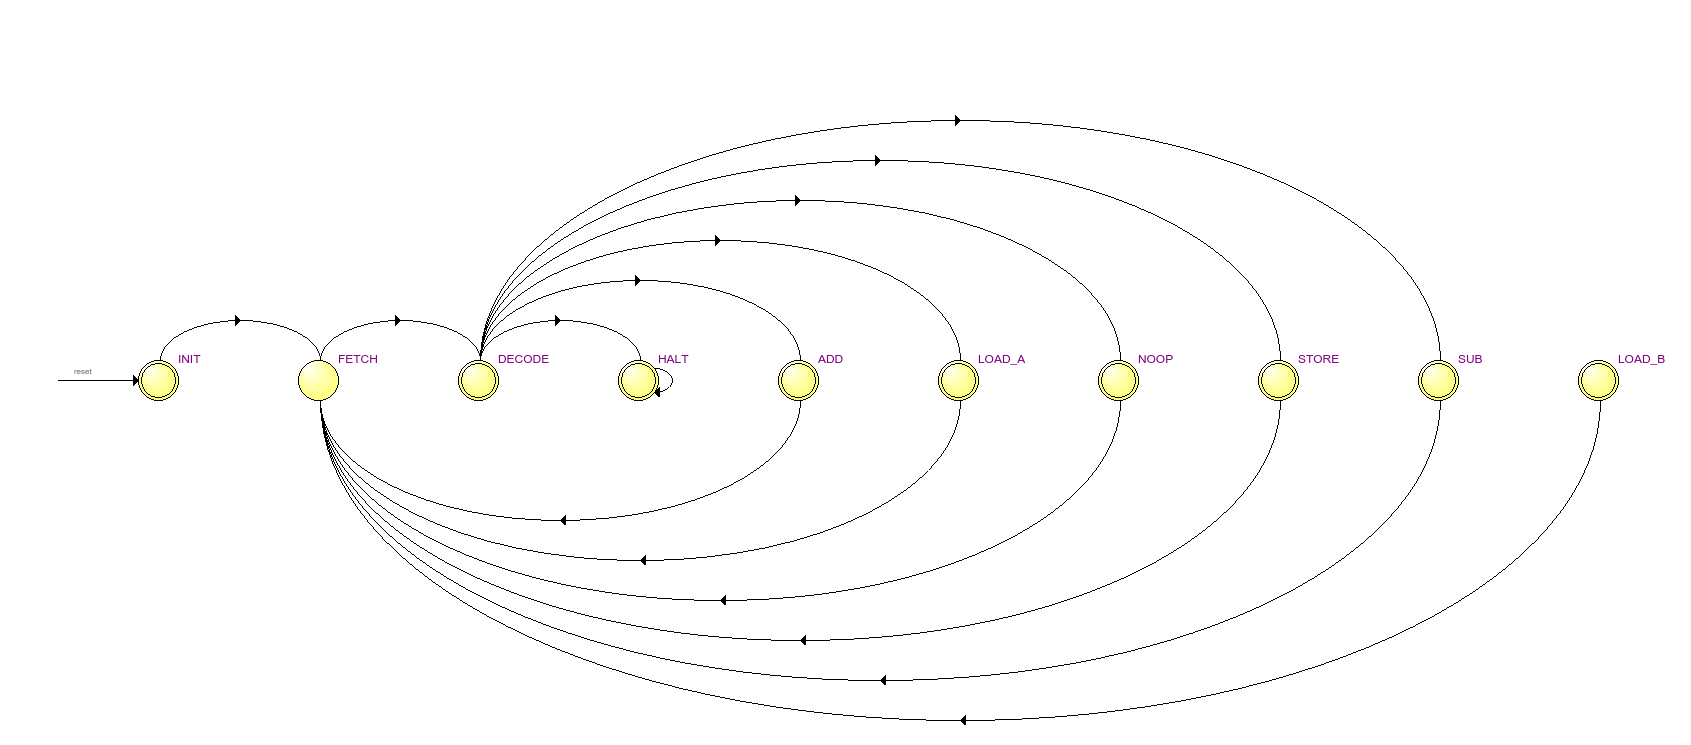
\includegraphics[width=\textwidth]{images/controller_rtl.png}
    \caption{Controller RTL View \label{fig:controller_rtl}}
\end{sidewaysfigure}

% subsection controller (end)

\subsection{Program Counter} % (fold)
\label{sub:program_counter}

The following observations correspond to the numbers in the \hyperref[sec:test_procedures]{Section \ref*{sec:test_procedures}} procedures for this part:

\begin{enumerate}
    \item The simulation using \emph{ModelSim} produced the output shown in \hyperref[fig:pc_output]{Figure \ref*{fig:pc_output}}.
    \item Sequantial values were generated when the count enable signal was high and the value was set to zero on a high reset signal.
\end{enumerate}

\begin{figure}[htbp]
    \begin{lstlisting}[numbers=none, basicstyle = \ttfamily\scriptsize]
# Time is          0 | Clock = 0 | Clear = 0 | O = 00
# Time is         10 | Clock = 1 | Clear = 0 | O = 01
# Time is         20 | Clock = 0 | Clear = 0 | O = 01
# Time is         30 | Clock = 1 | Clear = 0 | O = 02
# Time is         40 | Clock = 0 | Clear = 0 | O = 02
# Time is         50 | Clock = 1 | Clear = 0 | O = 03
# Time is         60 | Clock = 0 | Clear = 0 | O = 03
# Time is         70 | Clock = 1 | Clear = 0 | O = 04
# Time is         80 | Clock = 0 | Clear = 0 | O = 04
# Time is         90 | Clock = 1 | Clear = 0 | O = 05
# Time is        100 | Clock = 0 | Clear = 0 | O = 05
# Time is        110 | Clock = 1 | Clear = 0 | O = 05
# Time is        120 | Clock = 0 | Clear = 0 | O = 05
# Time is        130 | Clock = 1 | Clear = 0 | O = 05
# Time is        140 | Clock = 0 | Clear = 0 | O = 05
# Time is        150 | Clock = 1 | Clear = 0 | O = 05
# Time is        160 | Clock = 0 | Clear = 0 | O = 05
# Time is        170 | Clock = 1 | Clear = 0 | O = 05
# Time is        180 | Clock = 0 | Clear = 0 | O = 05
# Time is        190 | Clock = 1 | Clear = 0 | O = 05
# Time is        200 | Clock = 0 | Clear = 1 | O = 05
# Time is        210 | Clock = 1 | Clear = 1 | O = 00
# Time is        220 | Clock = 0 | Clear = 1 | O = 00
# Time is        230 | Clock = 1 | Clear = 1 | O = 00
# Time is        240 | Clock = 0 | Clear = 1 | O = 00
# Time is        250 | Clock = 1 | Clear = 1 | O = 00
# Time is        260 | Clock = 0 | Clear = 1 | O = 00
# Time is        270 | Clock = 1 | Clear = 1 | O = 00
# Time is        280 | Clock = 0 | Clear = 1 | O = 00
# Time is        290 | Clock = 1 | Clear = 1 | O = 00
    \end{lstlisting}
    \caption{Program Counter \emph{ModelSim} Output\label{fig:pc_output}}
\end{figure}

% subsection program_counter (end)

\subsection{Instruction Register} % (fold)
\label{sub:instruction_register}

The following observations correspond to the numbers in the \hyperref[sec:test_procedures]{Section \ref*{sec:test_procedures}} procedures for this part:

\begin{enumerate}
    \item The simulation using \emph{ModelSim} produced the output shown in \hyperref[fig:ir_output]{Figure \ref*{fig:ir_output}}.
    \item The register was loaded when the load enable signal was high and not when the load signal was low as expected.
\end{enumerate}

\begin{figure}[htbp]
    \begin{lstlisting}[numbers=none, basicstyle = \ttfamily\scriptsize]
# Time is          0 | input = 0000 | output = 0000
# Time is         20 | input = b0b0 | output = 0000
# Time is         30 | input = b0b0 | output = b0b0
# Time is         60 | input = d0d0 | output = b0b0
    \end{lstlisting}
    \caption{Instruction Register \emph{ModelSim} Output\label{fig:ir_output}}
\end{figure}

% subsection instruction_register (end)

\subsection{Processor} % (fold)
\label{sub:processor}

The following observations correspond to the numbers in the \hyperref[sec:test_procedures]{Section \ref*{sec:test_procedures}} procedures for this part:

\begin{enumerate}
    \item The simulation using \emph{ModelSim} produced the output shown in \hyperref[fig:processor_output]{Figure \ref*{fig:processor_output}}.
    This output is inconsistent with that expected.
    ALU
    \item All test vectors as specified in \hyperref[tab:processor_vectors]{Table \ref*{tab:processor_vectors}} produced the corresponding outputs
\end{enumerate}

\begin{sidewaysfigure}[htbp]
    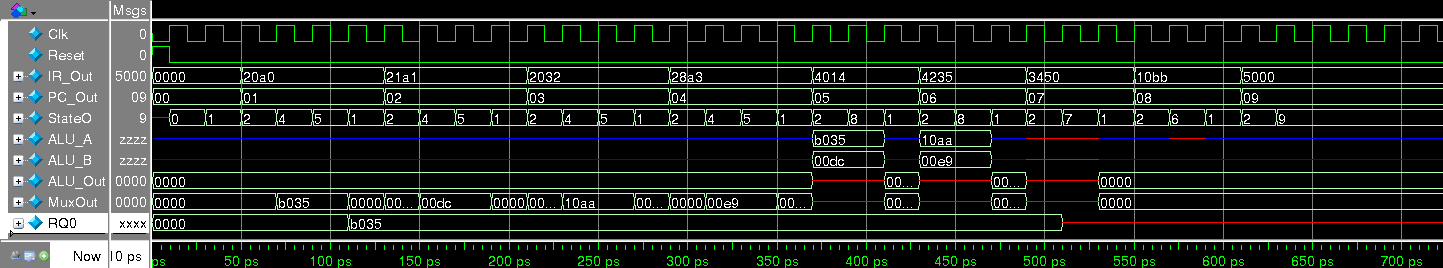
\includegraphics[width=\textwidth]{images/wave.png}
    \caption{Processor \emph{ModelSim} Output\label{fig:processor_output}}
\end{sidewaysfigure}

% subsection processor (end)

\subsection{Project} % (fold)
\label{sub:projects}

The following observations correspond to the numbers in the \hyperref[sec:test_procedures]{Section \ref*{sec:test_procedures}} procedures for this part:

\begin{enumerate}
    \item Compilation was successful, with the Flow Summary shown in \hyperref[lst:flow_summary]{Listing \ref*{lst:flow_summary}}.
    \item The project was downloaded to the DE2 board without errors.
    \item The displayed output was selectable as described in \hyperref[tab:display]{Table \ref*{tab:display}}.
\end{enumerate}

\lstinputlisting[basicstyle = \ttfamily\scriptsize, caption = \texttt{Flow Summary}, label = lst:flow_summary, numbers=none, keywords ={}]{flow_summary.rpt}

% subsection projects (end)

% section test_results (end) \FloatBarrier \clearpage
\FloatBarrier \section{Observations} % (fold)
\label{sec:observations}

The assignment was simplified by breaking it up into several simple modules.
Many of the modules could be repurposed from previous assignments.
The datapath module was built using an LPM RAM implementation and two modules from Homework 6.
The register file module had to be altered from the one used in Homework 6 to include the output of \verb|RF[0]|.
Since \verb|RegisterFile| was changed to output RQ0, then the \verb|RegisterOEN| module also had to be altered to output whatever contents were in the specified register.
In \verb|RegisterFile| however the only extra \verb|RegisterOEN| output that being used is the output from Register 0.

The program counter was very straightforward.
When compiling the program counter, \emph{Quartus} generates one warning in regards to the clear.
This is because the clear was hardcoded as one of the inputs to the multiplexer, and so it notes that it is stuck as ground.
However, this is intentional and is just an inherent part of the program counter, so the warning was ignored.
The reason the program counter was so simple for this lab was because there were no jump or branch instructions to deal with.
If there had been jump and branch instructions, the program counter would have needed an adder as well as additional logic to be able to change the given address accordingly.

Testing proved very difficult for this assignment.
We tried to simplify the process by testing many of the submodules individually.
This did prove very useful.
However, many processes which were successful on the DE2 board, would not function using \emph{ModelSim}.
At first, many errors were generated by output \verb|reg| types.
Though the DE2 would handle the correctly, \emph{ModelSim} would give them an initial value of \verb|x|.
This caused errors in several of our modules until we recognized the cause.
We were able to avoid this issue by using \verb|initial| statements to create initial values for all of our outputs.
The errors that we still see in \emph{ModelSim} may be from the LPM modules we used which we cannot initialize like our own modules.

We also had difficulties using LPM modules in \emph{ModelSim}.
We were finally able to figure out how to properly import them and where to import them from.
The \emph{Altera} LPM functions are not all held in the same \emph{ModelSim} library.
\emph{ModelSim} needs to import both \verb|220model_ver| and \verb|altera_mf|.

\emph{Quartus} reports tri-state errors in this project because the DE2 does not support internal tri-state wires.
\emph{Quartus} converts these internal tri-stated wires to selectors, and reports this change to us in a warning.
Instead of using the Z state out of the \verb|RegisterOEN| module, we can use a 0 output whenever read enable is not set.
If we do this, however, we then have 16 registers trying to write 0 to each output wire.
One cure for this is to build an OR gate.
The Verilog for this looks a bit unwieldy, as it contains 16 input wires OR-ed together.
This works because we only enable one register output at a time.
We initially implemented this method to avoid the tri-state errors, but \emph{ModelSim} was not able to properly recognize the circuit.

% section observations (end) \FloatBarrier \clearpage

\FloatBarrier \section{Conclusion} \clearpage

\FloatBarrier \phantomsection
\addcontentsline{toc}{section}{Appendix}
\section*{Appendix} \label{sec:appendix}

\lstlistoflistings \clearpage


\lstinputlisting[caption = \texttt{LabB.v}, label = lst:LabB]{../LabB.v}

\lstinputlisting[caption = \texttt{Pin Assignments}, label = lst:pins, numbers=none]{../atom_netlists/LabB.qsf}

\lstinputlisting[caption = \texttt{Hex7seg.v}, label = lst:hex]{../Hex7seg.v}

\lstinputlisting[caption = \texttt{Processor.v}, label = lst:processor]{../Processor.v}

\lstinputlisting[caption = \texttt{cunit.v}, label = lst:cunit]{../cunit.v}

\lstinputlisting[caption = \texttt{PC.v}, label = lst:pc]{../PC.v}

\lstinputlisting[caption = \texttt{PCAdder.v}, label = lst:PCAdder]{../PCAdder.v}

\lstinputlisting[caption = \texttt{muxlpm.v}, label = lst:muxlpm]{../muxlpm.v}

\lstinputlisting[caption = \texttt{instruction\_register}.v, label = lst:ir]{../instruction_register.v}

\lstinputlisting[caption = \texttt{controller.v}, label = lst:controller]{../controller.v}

\lstinputlisting[caption = \texttt{imemlpm.v}, label = lst:imemlpm]{../imemlpm.v}

\lstinputlisting[caption = \texttt{imem.mif}, label = lst:imemmif, keywords = {}, numbers = none]{../imem.mif}

\lstinputlisting[caption = \texttt{Datapath.v}, label = lst:datapath]{../Datapath.v}

\lstinputlisting[caption = \texttt{ramlpm.v}, label = lst:ramlpm]{../ramlpm.v}

\lstinputlisting[caption = \texttt{ramlpm.mif}, label = lst:rammif, keywords = {}, numbers = none]{../ramlpm.mif}

\lstinputlisting[caption = \texttt{RegisterFile.v}, label = lst:registerfile]{../RegisterFile.v}

\lstinputlisting[caption = \texttt{DecoderN.v}, label = lst:DecoderN]{../DecoderN.v}

\lstinputlisting[caption = \texttt{RegisterOEN.v}, label = lst:RegisterOEN]{../RegisterOEN.v}

\lstinputlisting[caption = \texttt{ALU.v}, label = lst:alu]{../ALU.v}

\lstinputlisting[caption = \texttt{testPCAdder.v}, label = lst:testPCAdder]{../testPCAdder.v}

\lstinputlisting[caption = \texttt{testPC.v}, label = lst:testPC]{../testPC.v}

\lstinputlisting[caption = \texttt{testinstruction\_register.v}, label = lst:testir]{../testinstruction_register.v}

\lstinputlisting[caption = \texttt{testProcessor.v}, label = lst:testProcessor]{../testProcessor.v}

\end{document}